\documentclass[senior,final,11pt]{iscs-thesis}
%論文の種類とフォントサイズをオプションに
%\usepackage{graphicx}% 必要に応じて
%\usepackage{mysettings}% 自分用設定

\pagenumbering{arabic} 

%-------------------
\etitle{Neural Network based Decompiler and its Evaluation}
\jtitle{ニューラルネットを用いた逆コンパイラとその評価}

__NAMES__

\date{February 1, 2018}
%-------------------


\newcommand{\argmax}{\mathop{\rm arg\,max}\limits}
%\newcommand{\argmin}{\mathop{\rm arg\,smin}\limits}

\usepackage{listings}
\usepackage{cite}
\usepackage{url}
\usepackage[numbers]{natbib}
\usepackage[dvipdfmx]{graphicx}
\usepackage{framed}
\usepackage{caption}

\lstdefinestyle{myCustomMatlabStyle}{
  language=C,
  numbers=none,
  stepnumber=1,
  numbersep=10pt,
  tabsize=2,
  showspaces=false,
  showstringspaces=false
}

\lstdefinestyle{Csample}{
  language=C,
  tabsize=2,
 	framesep=5pt,
}

\lstdefinestyle{Asmsample}{
  tabsize=2,
  framesep=5pt,
  %frame=none,
}

\lstdefinestyle{ForDecomp}{
  tabsize=2,
  frame=l,
  framesep=5pt
}


\lstset{%
  basicstyle={\small},%
  commentstyle={\small\itshape},%
  keywordstyle={\small\bfseries},%
  % style={myCustomMatlabStyle},
  stringstyle={\small\ttfamily},
  breaklines=true,
  columns=[l]{fullflexible},%
  % frame={tb},
  % numbers=left,%
  xrightmargin=0zw,%
  xleftmargin=3zw,%
  numberstyle={\scriptsize},%
  stepnumber=1,
  numbersep=1zw,%
  lineskip=-0.5ex,%
  captionpos=b,
}

\begin{document}
\begin{eabstract}
A decompiler is a tool for recovering a source code from compiled binary data.
There are various decompilers, but they often output a source code that is not intelligible to humans. 
In this thesis, we apply machine translation techniques to generate human intelligible decompiled source codes. 
More specifically, we propose to use recurrent neural networks with attention, 
which have been demonstrated to be useful for machine translation. 
In experiments, we use source codes collected from open source projects and their binary data for training and evaluating the neural networks.
From the experiment, we can observe little improvement in the result of decompilation with the use of attention.
Unfortunately, the results were not still good enough for practical use.

\end{eabstract}
\begin{jabstract}
逆コンパイラはコンパイル後のバイナリデータからソースコードを復元するためのツールである。
様々な逆コンパイラが存在するが、既存の逆コンパイラはしばしば人間にとって分かりにくいソースコードを出力する。
そこで本論文では、統計的機械翻訳の技術を逆コンパイラに用いた、解析者にとってわかりやすいソースコードを出力する逆コンパイラを提案する。
具体的には、機械翻訳において有用とされる注意機構付き再帰型ニューラルネットワークを用いる。
実験では、オープンソースプロジェクトから収集したソースコードとそのバイナリデータを用いてニューラルネットワークを学習し、その性能を検証した。
実験の結果、注意機構を用いることににより逆コンパイル結果における若干の精度向上が認められたが、実用的な精度までは至らなかった。
\end{jabstract}



\maketitle

\chapter*{Acknowledgement}
I thank Prof. Sugiyama and Lecture Sato for providing useful advice, supplying computational resources, helping me with writing this thesis and 
correcting my English.
I also thank A. Sano, who is my college classmate, for checking my English.

\tableofcontents

\chapter{Introduction}
% For dinamic analysis, malware is executed in the sandbox and the behavior is examined with the changes ocuuring in the sandbox. 
% Usually, there are two malware analysis approach, the dinamic analysis and the static analysis.
% In the static analysys, the behavior of the malware is analyzed by 

These days, the amount of malware has been increasing rapidly. In the report of AV-TEST Institute,
over 100 million malwares are newly found in every year for the past five years \citep{malware_increase}.
There are many case studies for malwareinfection \citep{malware_case_1,malware_case_2,malware_case_3,malware_case_4}.
In those cases, they analyse malwares to assess the impact of the incident and to identify the vulnerability which causes the infection.
% Therefore, the importance of developing malware analysis tools has been rising.
% 要参考文献 -> つけた。
In order to analyse malwares quickly and efficiently, there are some tools for analysing malwares \citep{mal_anal_tool}.
One of these tools is a decompiler, which is a tool for analyzing the behavior of malware. 
This tool generates a C-like pseudocode which represents the behavior of the malware, and analysts can infer the behavior of the malware from the pseudocode.
This is much easier compared to analyzing raw binary codes.

However, sometimes a decompiler generates an unstructured code, which requires users to make an effort to understand the behavior of the program. 
This is due to flexibility of the high level language. If the decompiler chooses a human-friendly representation of the language as a result of decompiling, we can analyze malware with less effort. 

In this thesis, we apply neural networks to the problem of decompilation to generate human-friendly pseudocodes. 
This idea is originated from \citet{Motoneta}, in which they used recurrent neural networks, in particular sequence-to-sequence model, for decompilation.
However, their model does not seem to be implemented some features for improving the quality of decompilation.
Therefore, we implemented the attention mechanism, which is introduced in \citet{dot_attention}, for improving the quality.
Additionally, the sequence-to-sequence model, which they used for the modeling, ignores the structure of a C language code.
Therefore, we also implemented the sequence-to-tree model, which is suggested in \citet{Seq2Tree}, for generating structured C language source code.

In the experiment, we tested three models, the basic sequence-to-sequence model, the sequence-to-sequence model with attention and the sequence-to-tree model.
As the result of the experiment, the attention mechanism showed little improvement in the performance, while the sequence-to-tree does not.
Unfortunately, the results of the all models were not still good enough for practical use.
The results of decompilation for short C source code fragment were not so bad. 
Nevertheless, the results for long C codes, which are considered to appear in practical use, were mostly failed.

% In the following part of the paper, we explain the 

\chapter{Related Works}
In this chapter, we review related works.

\section{Decompilation with Machine Learning}

Because perfect decompilation is naturally impossible, there are some machine learning applications for decompilation.

\citet{Motoneta} used the seqence-to-sequence model, which is a popular technique in the machine translation.
The seqence-to-sequence model is also evaluated in this thesis.

\citet{genetic_decompiler} applied genetic programming to decompilation.
They prepared a big corpus of C source codes, then they repeatedly mutated C codes to reduce the difference of the target binary and the compilation result of a C code. 

% TODO(satos)

% Compiler and Optimization Level Estimation for Improving Anti-malware Technologies

% 

\section{Improvement of decompilation results}
In this thesis, we do not try to recover the function name and variable name. 
However, for hand-decompilation, sometimes the name can be estimated from the functionality of the variable.
For example, \citet{hand_decompilation} used the Boomerang decompiler and repeatedly fixed variable types and names of the decompilation results 
to recover the source code of a software.

Here, we show a example of the name estimation.
Assume there is a variable X which seems to have a C struct type and has two fields P and Q.
Also, there are two functions F and G which operate with X. 
The function F receives X and another value V, assigns V to the memory indicated by P, adds 8 to P and increases Q. 
The function G receives X, subtracts 8 from P, decreases Q, and returns the value indicated by P.
In the situation, is is estimated that X,F and G have names related to {\sl stuck}, {\sl push} and {\sl pop}, respectively.

\citet{name_recover_from_decompile_result} tackled this work. 
In that paper, they tried to estimate the name of a variable which appears in the decompilation result of a compiled C program.

This kind of name estimation also appears in the context of deobfuscation.
\citep{deobfsucation_matome}
% これ雑にreferenceしたけどあんま意味ないよなぁ...?
Deobfuscation is a reverse process of obfuscation.
Obfuscation is a technique to modify the program source code so that the code becomes hard to understand for humans. 
Obfuscation is used for hiding the behavior of a program whose source code has to be distributed.
For example, in the web application, a JavaScript code of a program should be distributed in order to be executed on client web browsers.
Such JavaScript code is minified in order to protect the program from cracking. 
All comments, newlines, indents are removed and variable names are substituted to automatically generated meaningless names. 

\citet{JSNaughty} applied statistical machine translation for this task. 
They calculated the future value of a variable from its functionality, then 
sought the most suitable name from the candidates generated from the corpus.

% 変数の性質から統計情報を取り出し、それを元に

\section{Neural Network for Program Generation}

There are many applications of neural networks for program synthesis. They are summarized by \citet{deep_programming_matome}.

In this thesis, we applied sequence-to-tree model suggested by \citet{Seq2Tree}, 
because the input of the decompiler is a sequence of machine codes and
the output of the decompiler is an AST.

For another example, \citet{coffeescript_to_javascript} tried to mutually translate from JavaScript to CoffeeScript, and its inverse.
In that case, both JavaScript codes and CoffeeScript codes are tree structured, so they suggested tree-to-tree model.


\chapter{Problem Settings and Methods}

In this chapter, we explain a decompiler, its statistical formalization and 
the neural network models used in the experiment.
\section{Decompiler}

% 320 words.

A compiler is a program which compiles a source code written in language Y to another language X. 
% 文献 Usually, X is a high-level language and Y is relatively a low-level language. 
For example, a GNU C compiler translates the C language to the x64 assembly language, a javac compiler translates Java to a Java virtual machine code.
% This process is usually 
% 文献
% Especially, 
% This reverse process is usually insufficient or impossible.
A decompiler is a program which aims to reverse the process of a compiler, retrieving a source code of the high-level language Y from a source code of a low-level language X. 
When Y is a high-level language and X is relatively a low-level language, 
this reverse process becomes insufficient or impossible
\citep{hex_rays,decompile_hard_java}.
% for instance X is the C language and Y is the x64 assembly language 
This is because a lot of information, such as variable names or function names, is lost when compiling.
Additionally, the program structure described in the high level-language is lost too. 
For example, a simple \texttt{for} statement can be represented by the combination of a \texttt{while} statement and an \texttt{if} statement, or the combination of an \texttt{if} statement and a \texttt{goto} statement. 
So a decompiler cannot distinguish the difference in their representations, 
although in the real situation \texttt{for} statements are often used and \texttt{goto} statements are rarely used.



% これについてちゃんと書く。
% Their output psudecodes are sometimes wrong or hard to understand.

% (DONE)表がはみ出しているのでどうにかした。

% \let\oldlstinputlisting\lstinputlisting
% \renewcommand{\lstinputlisting}[2][]{\oldlstinputlisting[frame=lines,#1]{#2}}

\begin{figure}
	\begin{tabular}{cc}
		\begin{minipage}[c]{0.5\hsize}
		\fbox{
			\lstinputlisting[breaklines=false]{insert_list.c}
			}
			\caption*{Sample C source code}
		\end{minipage}
		\\ \\
		\begin{minipage}[b]{0.5\hsize} %title={Result of the Hopper Decompiler}
			\begin{framed}
			\lstinputlisting[]{snowman.c}
			\end{framed}
			\caption*{Result of the Snowman Decompiler}
		\end{minipage}
		\begin{minipage}[b]{0.5\hsize}
			\begin{framed}
			\lstinputlisting[breaklines=false]{recstudio.c}
			\end{framed}
			\caption*{Result of the REC Studio Decompiler}
		\end{minipage}
	\end{tabular}
	% \vspace*{-0.6cm}
	\caption{Decompilation results of existing decompilers for C source code}
	\label{fig:cw}
\end{figure}
Figure~\ref{fig:cw} shows an example of decompilation results of the Snowman decompiler version v0.1.3 and the REC Studio decompiler version 4.1 
for a sample C language code. The sample C code is compiled by the GNU C Compiler version 4.8.5, with the optimization level \texttt{-O0}.
The REC decompiler missed the structure of the variable \texttt{root}.
It also failed to estimate the number of arguments and the return value of the function.
The Snowman Decompiler succeeded in reconstructing the structure of the variable as \texttt{struct s0}.
It also succeeded in estimating the number of arguments and the return value as semantically correct expressions. 
However the statement \texttt{return 0;} is reconstructed to a complex combination of statements.

These incorrect or verbose results might be due to missing patterns in the assembly codes. 
Existing decompilers are made up with many steps similarly to compilers \citep{decompiler_path,hex_rays}.
In each step, a decompiler finds patterns in binary data, converts them to more high-level structure.
However, covering all patterns might be hardly possible, since there are many compilers and compiler optimizations \citep{hex_rays}.

By utilizing source code corpora, a statistical method might find patterns automatically, without enumerating each pattern.
Therefore, we will apply some statistical methods, which are described in the next section.

% These patterns comprehensive 

% The pathes are made up of 

% The \texttt{for} statement in the C source code is 
% reconstructed to the combination of the \texttt{while} statement and the {\sl if} statement in both decompiler results.

% This is the example of the impossibleness of the perfect decompilation, what we mentioned.



% However, there are many patterns 



% Existing decompilers are made up with many steps similarly to compilers. \citep{hex_rays,}
% They find patterns in binary data, convert them to more high-level structure, and chain them so that they can finally generate a high-level psudecode.



% このへん嘘書いてたので修正。
% The Hopper decompiler fails to detect while statements, and the variable {\sl now} is incorrectly analyzed.
% The output of snowman seems rather correct, as type {\sl struct tree} is reconstructed to {\sl struct s0}, 
% and the {\sl if} statement and {\sl while} statement are correctly restored. 
% However, it fails to detect the function epilogue, and the {\sl free} function call is incorrectly analyzed.
% Ideally, the decompilers can find correct function ranges and structure of statements, but they failed.


\section{Problem Settings and the Approaches}

% 189
In this thesis, we try to apply a statistical approach, specifically a statistical machine translation (SMT) technique, for decompilation.
SMT is the task which tries to translate one sentence $y$ written in one language into the sentence $x$ written in another language.

The decompilation problem is formulated as follows. 
Suppose that there is a compiler which converts a source code $ y $ written in one programming language 
to a source code $ x $  written in another programming language with probability $p(x|y)$.
In addition, suppose that $ y $ is a human-generated source code and follows the probability distribution $ p(y) $.
In this situation, the decompilation probability distribution $ p(y|x) $ is in proportion to $ p(x|y)p(y) $ according to the Bayes law, 
and $\argmax_{y} p(y|x)$ is considered as the best human-intelligible decompilation result for $x$.

In the experiment, we collected source codes from open source projects, which are regarded as the random sampling from the distribution $ p(y) $, 
and compiled them to generate the data pairs $ {\{(x_k,y_k)\}}_k $.
Then the data pairs are used for training the SMT models to estimate $p(y|x)$, and testing the performance of the models.

% Suppose that there is a compiler  Given $ x $ as a source code of domain language X, compiler generates $y$ as a code of target language Y with probability $p(sy|x)$.


% Given $x = [x_1, \dots, x_n] $ as a tokenized sequence of the source code of domain language X, compiler generates $sy$ as a code of target language Y with probability $p(sy|x)$.
% Then, the best decompilation result for target source code $sy$ is $ \argmax_{x} p(x|sy)$. 
% To generate $ \argmax_{x} p(x|sy)$, we decomposit $ p(x|sy) = p([x_1, \dots, x_n] |sy) = \prod_{k=1}^{n} p(x_k|sy,[x_1,\dots,x_{k-1}]) $,
% where $ p(x_k|sy,[x_1,\dots,x_{k-1}]) $ represents the probability that the token $ x_k $ follows to the sequence $ [x_1,\dots,x_{k-1}] $ 
% when the input sequence is $ sy $. 
% We try to estimate the probability $ p(x_k|sy,[x_1,\dots,x_{k-1}]) $ by LSTM, which is described in this section.
% With estimated $ p(x_k|sy,[x_1,\dots,x_{k-1}]) $, we can generate approximated $ \argmax_{x} p(x|sy)$ sequentially from $x_1$ to $x_n$ by selecting token $ \argmax_{x_{k}} p(x_k|sy,[x_1,\dots,x_{k-1}]) $ at each timing.

% The LSTM is 
% We assume the prior distribution $p(x)$ as the human-generated source code. 
% With that assumption, is in proportion to $p(sy|x)p(x)$ according to the Bayesian low, and 
% the $\argmax_{x} p(sx|y)$ is considered as the best human-intelligible decompilation result for the low-level code $y$.  
% So we try to estimate $ \argmax_{sx} p(y|sx)p(sx)$ for decompilation result.
% And if the compiler is deterministic, there would be a function $f$ which represents the compiler and $p(f(sx)|sx) = 1$,
% then the objective becomes to $ \argmax_{sx,f(sx)=y} p(sx)$.
% The distribution $p(sx)$ is approximated by collecting source code from open source projects.
% So if we had enough high-level source code data, we could choose the most popular high-level source code which generates given low-level code for the decompile result.
% However, high-level source code data can't be comprehensive.
% So we have to model the structure of compilation process somehow.
% We modeled the structure by the LSTM, which is commonly used in resent SMT techniques.

% (TODO)LSTM,Seq2seqの説明、その後Attentionについて説明、さらにその後seq2treeについて説明する。
\subsection{RNN and LSTM}
A recurrent neural network (RNN) is a neural network for dealing with sequence data.
The structure of the RNN is the sequence of the same node network units, as shown in Figure~\ref{fig:encoder} and Figure~\ref{fig:decoder}. 
The long short-term memory (LSTM) is a unit of the RNN which we used in the experiment. 
It was first introduced by \sloppy \citet{first_LSTM} , for overcoming the vanishing gradient problem and the exploding gradient problem.
In short, an LSTM unit receives two input vectors, 
one is the internal state of the LSTM unit, and the other is the input for the LSTM unit, 
and the LSTM unit emits one output vector, which represents the next internal state of the LSTM unit.

\subsection{Sequence-to-Sequence}
% This model is called seq2seq (sequence to seqence) model.

% 477 words.

The sequence-to-sequence model is the model for SMT task, introduced by \citet{seq2seq}.
% The combination of RNN and LSTM is applied to SMT task in, as the essential unit of the 
The sequence-to-sequence model is composed of two recurrent neural networks, the encoder network and the decoder network.

\begin{figure}[]
	\begin{center}
	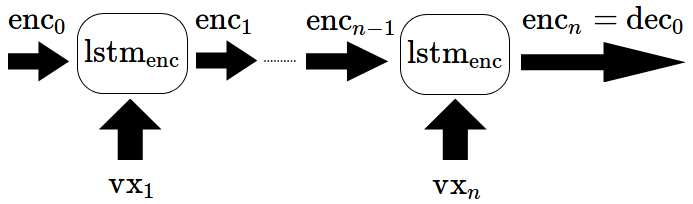
\includegraphics[height=3cm]{encoder.png}
	\end{center}
	\caption{The encoder network of the sequence-to-sequence model}
	\label{fig:encoder}
	\begin{center}
	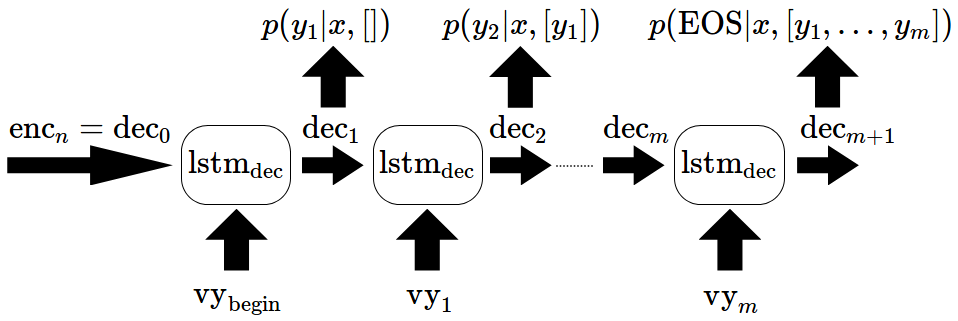
\includegraphics[height=4.2cm]{decoder.png}
	\end{center}
	\caption{ The decoder network of the sequence-to-sequence model}
	\label{fig:decoder}
\end{figure}

Figure~\ref{fig:encoder} shows the structure of the encoder network.  The purpose of the encoder network is to summarize the input sequence $x$, whose length varies depending on the sequence $x$, into a vector of fixed size.
This process is carried out as follows. 
First, $x$ is tokenized to sequence $x_{1} \dots x_{n}$, and each token $x_{k}$ is embedded to its vector representation $\mathrm{vx}_{k}$. 
Then, the initial LSTM internal state $\mathrm{enc}_0$ is initialized randomly, 
and $ \mathrm{enc}_{1} \dots \mathrm{enc}_{n} $ are calculated in accordance with the recursive formula $ \mathrm{enc}_{k} = \mathrm{lstm}_{\mathrm{enc}}(\mathrm{enc}_{k-1},\mathrm{vx}_{k}) $.
Finally, the last internal state $ \mathrm{enc}_{n}$ is returned as the reduced representation of the input sequence $x$.

Figure~\ref{fig:decoder} shows the structure of the decoder network.  The purpose of the decoder network is to estimate the distribution $ p(y_k|x,[y_1,\dots,y_{k-1}]) $ for each $ k $. 
The training process is carried out as follows. 
First, $y$ is tokenized, embedded to a vector representation $\mathrm{vy}_{1} \dots \mathrm{vy}_{m}$ in the same way as embedding $x$.
% prepended the token $ EOS $ for indicating the end of the sequence, then 
Then, the first internal state $ \mathrm{dec}_{1}$ is calculated from the start vector $\mathrm{vy}_{\mathrm{begin}}$ and encoded input $ \mathrm{enc}_{n} = \mathrm{dec}_{0} $ in accordance with the formula  $ \mathrm{dec}_1 = \mathrm{lstm}_{\mathrm{dec}}(\mathrm{dec}_{0},\mathrm{vy}_{\mathrm{begin}}) $.
Then, $ \mathrm{dec}_{2} \dots \mathrm{dec}_{m+1} $ are calculated in accordance with the recursive formula $ \mathrm{dec}_{k+1} = \mathrm{lstm}_{\mathrm{dec}}(\mathrm{dec}_{k},\mathrm{vy}_{k}) $.
Each decoder internal state $ \mathrm{dec}_{k} $ is passed to the linear layer $ W_{\mathrm{dec}} $ and then softmaxed to generate a probability vector $ \mathrm{py}_{k} = \mathrm{softmax}(W_{\mathrm{dec}}(\mathrm{dec}_{k}))$.
The probability vector $ \mathrm{py}_{k} $ is intended to represent the probability distribution $ p(y_k|x,[y_1,\dots,y_{k-1}]) $,
and last probability vector $ \mathrm{py}_{m+1} $ is intended to represent the probability of the end of the sequence $ p(\mathrm{EOS}|x,[y_1,\dots,y_{m}]) $.
Thus the network is trained to reduce the difference between predicted distribution $ \mathrm{py}_{k} $ and actual distribution $ p(y_k|x,[y_1,\dots,y_{k-1}]) $.
In the experiment, we chose cross-entropy of $ \mathrm{py}_{k} $ and $ p(y_k|x,[y_1,\dots,y_{k-1}]) $ as a loss function.

The inference from sequence $x$ is carried out by estimating
$ \argmax_{y} p(y|x) = \argmax_{y} \prod_{k=1}^n p(y_k|x,[y_1,\dots,y_{k-1}]) $.
Calculating argmax directly is exponentially time consuming, therefore we have to approximate the argmax by calculating $y = [y_1, \dots, y_m]$ sequentially.
First, $y_1$ is calculated as $ \argmax_{y_1} p(y_1|x,[]) $, where the distribution $ p(y_1|x,[]) $ is approximated by 
$ \mathrm{softmax}(W_{\mathrm{dec}}(\mathrm{dec}_{1}))$. 
Then, the next token $y_2 = \argmax_{y_2} p(y_2|x,[y_1]) $ is calculated from $ \mathrm{dec}_{1} $ and the vector embedding of $y_1$, and so on.
When the token $y_{m+1}$ is the EOS token, the generating process is stopped and the sequence $ [y_1, \dots ,y_m]$ is returned as an inference result.

% ビームサーチ書く。
% For TODO

% (TODO) このへんで 図を入れる
% (TODO) 理由/気持ち について述べたいですね。

What is mentioned above is the basic structure of the sequence-to-sequence model.
To improve the performance of the sequence-to-sequence model, there are some devices for the model.
In the following, we introduce two devices, which are used in our experiment.

The first is the bidirectional RNN (BRNN), which is the architecture introduced by \citet{BiRNN}.
In our experiment, this architecture is used for the encoder network as follows.
In addition to the internal state $ \mathrm{enc}_{k} $, the reverse internal state $ \mathrm{enc}_{k}^{\gets} $ is also calculated 
in accordance with the recursive formula $ \mathrm{enc}_{k}^{\gets} = \mathrm{lstm}_{\mathrm{enc}}^{\gets}(\mathrm{enc}_{k+1}^{\gets},\mathrm{vx}_{k}) $.
Then both of the internal states $ \mathrm{enc}_{n} $ and $ \mathrm{enc}_{0}^{\gets} $ are used for the decoder network.

The second is the multi-layer RNN, introduced by \citet{multi_layer}.
They reported that, feeding the output sequence of one LSTM network to another LSTM network, similarly to stacking the network layers, will improve the accuracy of prediction.
This architecture is called the stacked RNN or the multi-layer RNN.



% It is reported that, instead of the output of the LSTM units to another LSTM units will improve the accuracy of the prediction.
% This architecture is called as stucked reccurent neural networks or multi-layer reccurent neural networks.


\subsection{Attention}
Attention is an extension module for the sequence-to-sequence model to improve the quality of translation. 
A simple sequence-to-sequence model has a problem that the size of the encoded vector $enc_{n}$ is fixed 
regardless of the length of the input sequence $x$. 
Therefore, the longer the length of the input becomes, the more likely the information of the input will be lost.
This problem is eased by using the information in the encoding network when decoding the output sequence.

The attention module was first developed by \citet{attention_paper}.
We implemented the global general attention, which was introduced by \citet{dot_attention}, for improving the quality of decompilation.
In the following, we will describe the global general attention.

As the mentioned in the previous section, the pure sequence-to-sequence model uses the output of the decoder network $ \mathrm{dec}_{k} $ for estimating 
the distribution $ p(y_k|x,[y_1,\dots,y_{k-1}]) $.
In the sequence-to-sequence model with attention, 
a context vector $ \mathrm{ctx}_{k} $ is calculated from $ \mathrm{dec}_{k} $ and the internal states of encoder networks $ \mathrm{enc}_{1} \dots \mathrm{enc}_{n} $, 
then the distribution is estimated from the output vector $ \mathrm{dec}_{k} $ and context vector $ \mathrm{ctx}_{k} $.
The context vector $ \mathrm{ctx}_{k} $ is calculated as follows.
For each encoder state $ \mathrm{enc}_{l} $, the importance of the state is calculated as $ a_{l} = \mathrm{score}(\mathrm{dec}_{k},\mathrm{enc}_{l}) $,
then $ \mathrm{ctx}_{k} $ is calculated as $ \mathrm{ctx}_{k} = \sum_{l=1}^{n} \frac{\exp{a_{l}}}{\sum_{l=1}^{n}\exp{a_{l}}} \mathrm{enc}_{l} $, 
as the weighted average of $ \mathrm{enc}_{1} \dots \mathrm{enc}_{n} $.
% Multiple score functions are introduced by \citet{dot_attention}, and we choiced 
In \citet{dot_attention}, various kinds of score functions were suggested.
In our experiment, we used a general score function, which is calculated as $ \mathrm{score}(\mathrm{dec}_{k},\mathrm{enc}_{l}) = \mathrm{dec}_{k}^T W \mathrm{enc}_{l} $ ,
where $ W $ is a parameter matrix.

% With the information of the internal state $ \mathrm{ctx}_{k} $ of the encoder network, the decoder network can access to the 

% アテンション機構を用いる場合、前述したようにdecoder networkの出力 $ dec_{k} $ をそのまま用いて分布をesitmateするのではなく、
% $ dec_{k} $ と encoder network の出力 $ enc_{1} \dots enc_{n} $ (encoder が BiLSTMの場合 $ enc^{\gets}_{1} \dots enc^{\gets}_{n} $ も)
% を用いて context vector $ \mathrm{ctx}_{k} $ を生成し、 $ dec_{k} $ と $ \mathrm{ctx}_{k} $ によって条件付き分布をesitmateする。

% $ \mathrm{ctx}_{k} $ は、 $ enc_{1} \dots enc_{n} $ の加重平均によって計算される。 具体的には、
% 各状態 $ enc_{l} $ について その状態のスコア $ a_{l} = score(dec_{k},enc_{l}) $ を計算し、
% $ \mathrm{ctx}_{k} = \sum_{l=1}^{n} \frac{\exp{a_{l}}}{\sum_{l=1}^{n}\exp{a_{l}}} enc{l} $ として計算される。

% この $ \mathrm{ctx}_{k} $ を併せて用いることにより、 分布予測時に入力データの情報にアクセスすることができ、精度の向上が見込める。


% In the pure sequence-to-sequence model, the conditional probability  $ p(y_k|x,[y_1,\dots,y_{k-1}]) $ is calculated from $ dec_{k} $ ,which is the internal state of the decoder network.
% In the sequence-to-sequence with attention model, the probability is calculated from $ dec_{k} $ and the context vevctor $ c_{k} $.
% $ c_{k} $


% After generating $ dec_{k} $, the context vector $ c_{k} $ is calculated from the hidden states $ enc_{1} \dots enc_{n} $.

% $ c_{k} = \sum_{k=1}^{n} $ 

% The attentional hidden state $ dec'_{k} $ is calculated from the $ dec_{k} $ and $ c_{k} $.
% Then, the probability $ p(y_k|x,[y_1,\dots,y_{k-1}]) $ is estimated as $ \mathrm{softmax}(W_{dec}(dec'_{k}))$, instead of $ \mathrm{softmax}(W_{dec}(dec_{k}))$.




\subsection{Sequence-to-Tree}
% 184 words
Compared to natural languages, programming languages obey rigid grammars. % wich are usually context free grammers.
Therefore, it is reasonable to consider the grammar of the programming language when generating programs.
Sequence-to-tree is a model for generating a tree-structured output from a sequence input. 
This model was introduced by \citet{Seq2Tree} for generating a program from a program specification written in natural language. 
This task is similar to our task which aims to generate programs from assembly codes, which are sequences of instructions.
Therefore we implemented this model in the experiment.

Now, we will describe the sequence-to-tree model.
The sequence-to-tree model is composed of two networks, the encoder network and the decoder network.
The encoder network of the sequence-to-tree model is the same as that of the sequence-to-seequence model. 
It summarizes an input sequence into a vector of fixed size.

\begin{figure}[]
	\begin{center}
	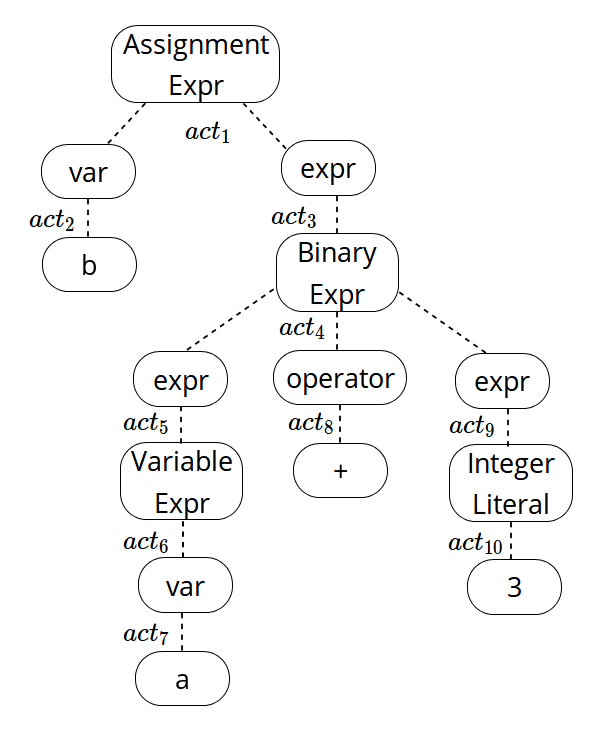
\includegraphics[height=11.5cm]{ast_zu.png}
	\end{center}
	\caption{abstract syntax tree (AST) representation of a C statement \texttt{b = a + 3;} }
	\label{fig:ast_zu}
\end{figure}

The decoder network is a network for generating tree structured output. 
A tree structure is representable by a sequence of the actions which expands a nonterminal symbol of the constructing tree.
For example, the tree shown in Figure~\ref{fig:ast_zu} is generated from the sequence $ [\mathrm{act}_1, \dots, \mathrm{act}_{10}] $, 
where action $ \mathrm{act}_k $ expands the left-most nonterminal symbol in the tree generated from the action sequence $ [\mathrm{act}_1, \dots, \mathrm{act}_{k-1}] $. 
Suppose the tree $t$ is generated by the action sequence $ [\mathrm{act}_1, \dots, \mathrm{act}_m] $, 
then the tree-generating probability $ p(t|x) $ is decomposed into $ \prod_{k=1}^n p(\mathrm{act}_k|x,[\mathrm{act}_1, \dots, \mathrm{act}_{k-1}]) $. 
Thus the sequence-to-sequence model is now applicable to generating tree structure, by embedding each action $\mathrm{act}_k$ to represent vector $\mathrm{av}_k$ and 
calculate $ \mathrm{lstm}_{\mathrm{dec}}(\mathrm{dec}_{k},\mathrm{av}_{k}) $ sequentially for estimating $p(\mathrm{act}_{k+1}|x,[\mathrm{act}_1, \dots, \mathrm{act}_{k}]) $.  

% In algorithmic parspective, the inference of the seq2seq model tries to generate sequence one by one, from the first token to the last.
% The Seq2Tree model also tries to generate tree structure one by one, with depth-first order.
% The inference of the SeqTree model starts from the start symbol, and recursively expand the nonterminal symbols in depth-first order.

In the sequence-to-tree model, the information which is peculiar to the tree structure is additionaly used.
For expanding node $d$, the information of the node type $ \mathrm{nf}_{d} $ and the parent action $\mathrm{pa}_{d}$ from which node $d$ is generated is used.
Then the next internal state is calculated as $ \mathrm{lstm}_{\mathrm{dec}}(\mathrm{dec}_{k},[\mathrm{av}_{k}; \mathrm{nfv}_{d}; \mathrm{pav}_{d}]) $ instead of $ \mathrm{lstm}_{\mathrm{dec}}(\mathrm{dec}_{k},\mathrm{av}_{k}) $, 
where $\mathrm{nfv}_{d},\mathrm{pav}_{d}$ are the vector embeddings of $\mathrm{nf}_{d},\mathrm{pa}_{d}$.

In \citet{Seq2Tree}, they also used a devised method for generating terminal symbols, because they need to copy the name of some variables from the program specification.
However, in our case, we do not need to copy the information from the input, because the name information is lost when compiling.
Nevertheless, it was found from our preliminary experiments that our models often fail to recover the constant values in the programs.
Therefore, implementing the copying method for values is left as future work.

% しかしながら、実験の結果、ソースコード中の定数に関しては復元が困難であることが観察された。このため、プログラム中の定数に関してこのcopy method を実装することが考えられるが、
% これは future work とする。

% \subsection{Path Decomposite Sequence-to-Tree}
% 前述の Sequence-to-Tree は プログラムの構造を考慮しているものの、アクションをそのまま列にするのは結局プログラムの木としての構造がある程度失われてしまっているのではないかと考えられる。
% すなわち、アクションを列に展開しているため、ある部分木からその兄弟の部分木の生成に移る際に大幅なジャンプが生じている。

\chapter{Evaluation Experiment}
In this chapter, we explain the details of the evaluation experiment.
% In this chapter, we show the evaluated result of the three models, Seq2Seq, Seq2SeqAtt, and Seq2Tree.
The source codes for the experiment are available at \url{https://github.com/satos---jp/neural_decompiler}.  

\section{Data Collection}
% 219 words
We collected source codes from GitHub \citep{github} by crawling.
We cloned about 900 repositories with the C language topic, 
and recursively searched each repositoriy to enumerate C language source codes.
From each source code, we generated pairs of a C source code fragment and an x64 assembly code corresponding to the C source code fragment.
Some example data pairs are shown in Figure~\ref{fig:pairsoffragments}. 

\begin{figure}
	\begin{tabular}{|l|l|} \hline
	 C source code & x64 assembly \\ \hline 
		\begin{lstlisting}[style=Csample]
		r *= a
		\end{lstlisting}
		&
		\begin{lstlisting}[style=Asmsample]
	mov eax,DWORD [rbp-0x4]
	imul eax,DWORD [rbp-0x14]
	mov DWORD [rbp-0x4],eax
		\end{lstlisting} \\ \hline	
		\begin{lstlisting}[style=Csample]
	while(p >= 0){
		p--;
		r *= a;
	}
		\end{lstlisting}
		&
		\begin{lstlisting}[style=Asmsample]
	jmp LABEL_0
LABEL_1 :
	sub DWORD [rbp-0x18],0x1
	mov eax,DWORD [rbp-0x4]
	imul eax,DWORD [rbp-0x14]
	mov DWORD [rbp-0x4],eax
LABEL_0 :
	cmp DWORD [rbp-0x18],0x0
	jns LABEL_1
		\end{lstlisting} \\ \hline		
		\begin{lstlisting}[style=Csample]
int pow(int a,int p){
	int r = 1;
	while(p >= 0){
		p--;
		r *= a;
	}
	return r;
}
		\end{lstlisting}
		&
		\begin{lstlisting}[style=Asmsample]
	push rbp
	mov rbp,rsp
	mov DWORD [rbp-0x14],edi
	mov DWORD [rbp-0x18],esi
	mov DWORD [rbp-0x4],0x1
	jmp LABEL_0
LABEL_1 :
	sub DWORD [rbp-0x18],0x1
	mov eax,DWORD [rbp-0x4]
	imul eax,DWORD [rbp-0x14]
	mov DWORD [rbp-0x4],eax
LABEL_0 :
	cmp DWORD [rbp-0x18],0x0
	jns LABEL_1
	mov eax,DWORD [rbp-0x4]
	pop rbp
	ret
		\end{lstlisting} \\ \hline
	\end{tabular}
	\caption{Example of training data pairs}
	\label{fig:pairsoffragments}
\end{figure}

These pairs were generated as follows. Let S0 be an original C source code.
\begin{enumerate}
\item Remove all preprocessors, such as \texttt{\#include}, in S0 to generate preprocessed C code S1. 
\item Tokenize S1 and rearrange into S2 so that there is exactly one token for each line. 
\item 
Compile S2 by the GNU C compiler with no optimization option (-O0) and debug option (-g) to get assembly code S3. 
With the debug option, S3 contains the information about the corresponding source code positions in S2. 
% which each assembly operations are originated from.
\item Assemble S3 to object file S4 and disassemble S4 to get information eliminated assembly code S5.
\item 
Parse S2 with a Clang compiler to get the abstract syntax tree (AST) of the source code and enumerate the subtrees of the AST.
Each subtree of the AST has the corresponding source code positions in S2.
Therefore, we can get a pair of an assembly code and a C fragment corresponding to the subtree 
by using the informations in S2, S3 and S5.
\end{enumerate}

The pairs of a C fragment and an assembly code are then preprocessed for the training and the testing data.

\section{Data Preprocessing}

% 34 words
In order to apply the sequence-to-sequence model, 
we have to preprocess the assembly codes and the C fragments into the sequences of tokens.

\subsection{Assembly Code Preprocessing}
% 155 words
There are two ways for preprocessing assembly codes.

The first way is converting each code into the sequence of integers. 
In order to execute as a program, an assembly code is assembled into the sequence of one-byte integers, ranging from 0 to 255.
Therefore the one-byte integer sequences can be directly used as input sequences to the sequence-to-sequence model.

The second way is converting each code into the tokenized sequence of assembly codes. 
That is, we split the disassembled instructions in S5 into the sequence of symbols, 
concatenate these sequences to one sequence, 
and modify it as follows:
\begin{itemize}
\item For each end of the instructions, the \texttt{ENDLINE} token is added to indicate the end of the instructions.
\item 
The relative addressing, such as the address of the \texttt{call} or \texttt{jump} instructions, 
is normalized by renaming so as to make the code position independent and to reduce the vocabulary size.
\item Big integer values are clipped. 
More specifically, an integer in the range from -255 to 256 are preserved as it is, and other integers are clipped and substituted with the \texttt{\_\_HEX\_\_} symbol.
This also reduces the vocabulary size.
\end{itemize}

We chose the second way for the experiment.
This is because, in our case, the assembly code is generated from the GNU C compiler, which is a common compiler.
Therefore the assembly code can be disassembled uniquely.
For example, \citet{disasm_obfuscate} proposed an obfuscation technique, which deceives a disassembler to generate wrong disassembly results.
In that case, the first way might be better than the second way.

\subsection{C Code Preprocessing}
% 232 words
The C source codes were parsed to AST by a Clang compiler \citep{clang} and its Python bindings together with pycparser \citep{pycparser}, 
because all of the tools are individually not sufficient for generating a dataset.
Then, the AST is converted to input data as follows:

\begin{itemize}
\item The variable-ary nodes and optional nodes were converted. 
For example, the \texttt{CompoundStatement} node has a variable number of statements. 
We converted such a list of nodes to the chains of the node \texttt{CONS} and the node \texttt{NIL}, as the list representation in a functional language.
Another example is the \texttt{if} statement, whose \texttt{else} clause is sometimes missing. 
We converted such optional nodes to the alternative of the \texttt{SOME} node and the \texttt{NONE} node, as the optional data structure in a functional language.
\item The variable names, function names, label names, or type names were renamed similarly to the addresses in the assembly code data.
\item There are four type of literals in the C language. 
An integer literal less than 256 was preserved, and an integer literal greater than 256 was clipped to 256.
The string, float and character literals were converted to the \texttt{\_\_LITERAL\_\_} symbol.

% Modifying the node to indicate the value in the assembly code corresponding to the literal is also conceivable way,
% but we did not implement this because of its technical difficulty, so this is left to future work.
\end{itemize}

ASTs were used for the sequence-to-tree model as they were, or converted to C token sequences for the sequence-to-sequence model. 

\section{Model Configuration}
The training model was implemented with Chainer version 4.5.0 \citep{chainer}.
We implemented three models, Seq2Seq, Seq2SeqAtt, and Seq2Tree.

The encoder network was a bidirectional LSTM in all of the three models.
The decoder network of Seq2Seq and Seq2SeqAtt predict the conditional probability of the next token $ p(y_k|x,[y_1,\dots,y_{k-1}]) $,
while the decoder network of Seq2Tree predicts the conditional probability of the next action $ p(\mathrm{act}_{k}|x,[\mathrm{act}_1, \dots, \mathrm{act}_{k-1}]) $.

Seq2SeqAtt and Seq2Tree are the models with attention, while Seq2Seq is not.

\begin{figure}[t]
	\caption{The configuration parameters of the models}
	\begin{tabular}{|c||c|c|c|}
		\hline
		  & Seq2Seq & Seq2SeqAtt & Seq2Tree \\ \hline \hline
		 Generate & \multicolumn{2}{|c|}{token sequence} & AST \\ \hline
		 With Attention & no & \multicolumn{2}{|c|}{yes} \\ \hline
		 Encoder & \multicolumn{3}{|c|}{Bidirectional LSTM} \\ \hline
		Number of LSTM Layers & \multicolumn{3}{|c|}{4} \\ \hline
		Dimensionality of Vector Embedding & \multicolumn{3}{|c|}{128} \\ \hline
	\end{tabular}
	\label{fig:parameterofmodels}
\end{figure}

Figure~\ref{fig:parameterofmodels} shows the parameters of the models. 

% (TODO)レイヤ数、ロスについてのべる。

\section{Model Training}
% 91 words
We trained these models to reduce the cross-entropy loss between predicted and actual conditional probabilities.
The conditional probability is the probability of next token $ p(y_k|x,[y_1,\dots,y_{k-1}]) $ for the sequence-to-sequence model, 
and the probability of next action $p(\mathrm{act}_{k+1}|x,[\mathrm{act}_1, \dots, \mathrm{act}_{k}]) $ for the sequence-to-tree model.

For the optimizer of the training, we used Adam, which was introduced by \citet{Adam}.
The parameters of Adam were set to $ (\alpha,\beta_1,\beta_2) = (0.001,0.9,0.999) $, which are the default parameters of Chainer version 4.5.0.
% 学習の際のoptimizerにはAdam(文献)を用いた。

\section{Evaluation Metrics}
We evaluated the quality of the results by two metrics, 
the edit distance ratio \citep{Motoneta} and the bilingual evaluation understudy (BLEU) \citep{BLEU}.

The edit distance ratio is a metric for for the correctness of the decompilation result.
Here, the edit distance ratio between two strings means the Levenshtein distance \citep{levensthein_dist} divided by the length of the longer string.
Ideally, the correctness of the decompilation result should be measured by the distance of the meaning of the program.
However the decompilation result is usually uncompilable, 
thus we used the edit distance of the source codes as an approximation of the correctness.

BLEU is the metrics for the similarity of the ground truth and the decompilation result. 
It was first introduced by \citet{BLEU}, for evaluating the performance of machine translation.
BLEU is calculated from the sets of n-grams for each sentence. 
If the two sentences have similar n-gram sets, the BLEU score becomes higher.
In our case, it means that the decompilation result is more similar to the program written by human. %, that is, more human intelligible.

% 2つの文のn-gram集合が似ているほど、BLEUスコアは高くなります。今回の場合はデコンパイル結果がより人間らしい自然な出力となっていることを意味します。

Before calculating these scores, we normalized variable names in the source codes by renaming.
% 補足として、今回は edit distance と BLEU を計算する際に、変数名を先頭から順に順番に付け直すことにより、ソースコード中の変数名の付けなおしを行っている。
% これはプログラムの意味は変数名に依らないためである。

% \chapter{Evaluation}
% In this chapter, we show the evaluated result of the three models, Seq2Seq, Seq2SeqAtt, and Seq2Tree.
% We trained each models with reedbush, を用い、各モデルについて4時間学習させた。
% We collected approximately $ 10^7 $ pairs of datasets. 

% \section{Furure work}

% TODO(satos)

% At first, we show the 

% まず先に、学習に用いたデータ長の分布を Figure~\ref{fig:editdist} に示す。
% ソースコードの部分木を全て列挙するデータ生成法の性質上、長さの短いコード辺が極端に多いことが確認できる。

% We tested three models. 

% 今回、それぞれのモデルの学習には、東京大学のreedbushを用い、各モデルについて4時間学習させた。

% 精度計測では、各モデルに対して テストケースから100個のデータをランダムに取り出して翻訳させ、それらの編集距離とBLEU値の平均を計測した。

\section{Numerical Evaluation}
In order to evaluate each model, we randomly sampled 100 data pairs from test cases.
For each test case, we generated decompilation results from the assembly code data of the test case.
Then, we averaged the edit distance ratios and BLEU scores between results and ground truths.

\begin{figure}[]
	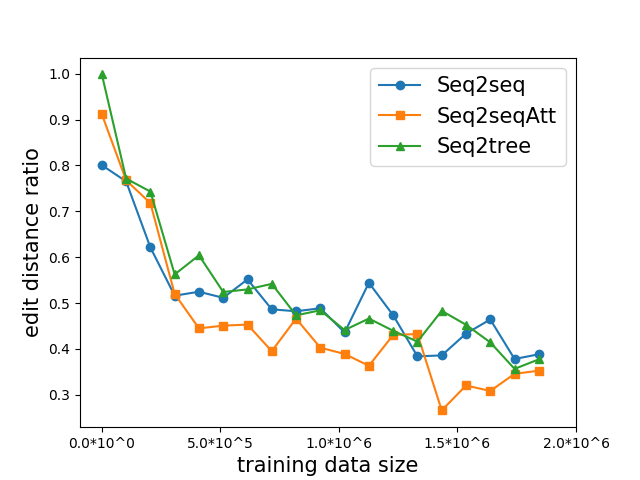
\includegraphics[width=12cm]{edit_dist.png}
	\caption{Averaged edit distance ratio for each models}
	\label{fig:editdist}
	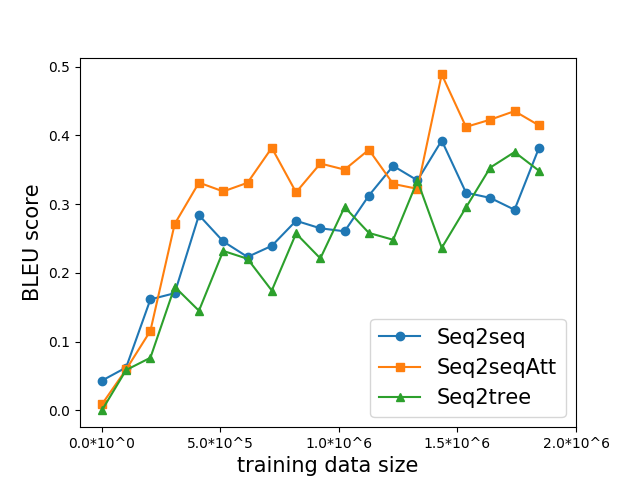
\includegraphics[width=12cm]{bleu.png}
	\caption{Averaged BLEU score for each models}
	\label{fig:bleu}
\end{figure}

% 図1は各モデルについて、学習に用いたデータ数と編集距離をプロットしたグラフである。
% 図2は各モデルについて、学習に用いたデータ数と編集距離をプロットしたグラフである。
Figure~\ref{fig:editdist} shows the relation between the training data size and the averaged edit distance ratio for each model.
Figure~\ref{fig:bleu} shows the relation between the training data size and the averaged BLEU score for each model.
The lower edit distance ratio and the higher BLEU score mean better decompilation performance.

We can see that Seq2SeqAtt shows slightly better results in both the edit distance ratios and BLEU scores,
 which implies that the attention improves the performance of the decompilation.
However, there is no significant difference between Seq2Seq and Seq2Tree in both metrics.
This seems to be due to the length of the sequences to be estimated.
% Seq2seqの結果とSeq2seqAttの結果を比較することにより、attention が性能向上に寄与していることがわかります。
% 逆にSeq2treeにはattentionがあるにもかかわらずSeq2seqと比較して性能向上が見られなかったわけですが、
% これはCのソースコードをASTに変換した際に、データサイズが増えたためであると考えられます。

\begin{figure}[]
	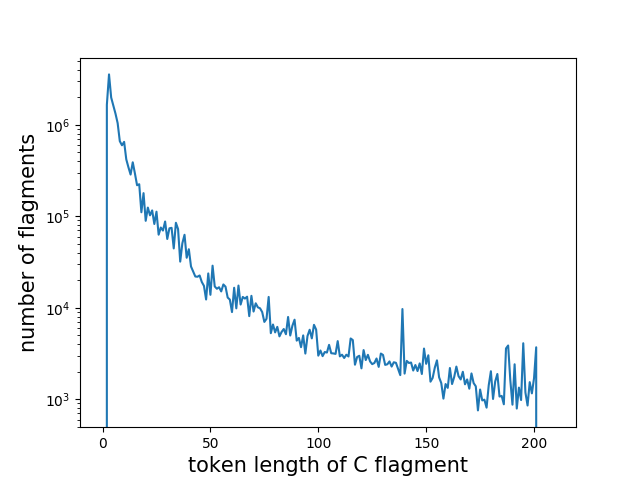
\includegraphics[width=12cm]{c_lens.png}
	\caption{Length distribution of C token fragments}
	\label{fig:csizes}
	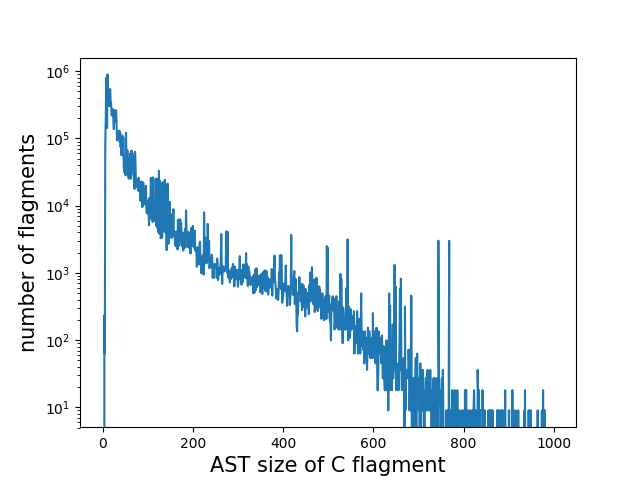
\includegraphics[width=12cm]{ast_lens.png}
	\caption{Length distribution of datasets as AST}
	\label{fig:astsizes}
\end{figure}

Figure~\ref{fig:csizes} shows the length distribution of the dataset as C token sequences, 
and Figure~\ref{fig:astsizes} shows the size distribution of the same dataset as ASTs.
The size of an AST is equal to the length of its action sequence.
According to these two figures, the AST size is 2 or 3 times larger than the length of C token sequences.
Therefore, the AST estimation may be harder than the C token sequence estimation.

\begin{figure}
	\begin{tabular}{|l|l|} \hline
	 ground truth & 
		\begin{lstlisting}[style=Csample]
r *= a
		\end{lstlisting} \\ \hline
		Seq2Seq & 
		\begin{lstlisting}[style=Csample]
const unsigned int V0 = V1 * floatliteral
		\end{lstlisting} \\ \hline
		Seq2SeqAtt & 
		\begin{lstlisting}[style=Csample]
V0 = ( unsigned int ) ( V1 ) * ( unsigned int ) V2
		\end{lstlisting} \\ \hline
		Seq2Tree & 
		\begin{lstlisting}[style=Csample]
V0 = V0 * V1
		\end{lstlisting} \\ \hline
		\hline	
	 ground truth & 
		\begin{lstlisting}[style=Csample]
while(p >= 0){
	p--;
	r *= a;
}
		\end{lstlisting} \\ \hline
		Seq2Seq & 
		\begin{lstlisting}[style=Csample]
for(;V0 = (1<<(((unsigned int)-1<<((32-20)-1))-1))
*((unsigned char*)(V1.V2))[1] = (unsigned char)2;
}
		\end{lstlisting} \\ \hline
		Seq2SeqAtt & 
		\begin{lstlisting}[style=Csample]
while(((void *) >= 0) != ((void *) 0)){ 
	return ((void *) 0);
} else { 
	V0 = (( void * ) 0); 
}
		\end{lstlisting} \\ \hline
		Seq2Tree & 
		\begin{lstlisting}[style=Csample]
while(V0 < 0){ 
	V1 = V0 - 1;
}
		\end{lstlisting}
		 \\ \hline	\hline
	 ground truth & 
		\begin{lstlisting}[style=Csample]
int pow(int a,int p){
	int r = 1;
	while(p >= 0){
		p--;
		r *= a;
	}
	return r;
}
		\end{lstlisting} \\ \hline
		Seq2Seq & 
		\begin{lstlisting}[style=Csample]
void V0(int V1,int V1){ 
	int V1 = 0; 
	int V1; 
	for(V2=1;V1<=V2;++V2){ 
		V1 = * V3; 
	} 
}
		\end{lstlisting} \\ \hline
		Seq2SeqAtt & 
		\begin{lstlisting}[style=Csample]
void V0(unsigned int V1,unsigned int V2){ 
	unsigned int V1 = ((void *) 0); 
	unsigned int V3 = ((void *) 0); 
	unsigned int V1 = ((((void *) 0) != ((void *) 0))); 
	return V4; 
}
	\end{lstlisting} \\ \hline
		Seq2Tree & 
		\begin{lstlisting}[style=Csample]
INVALID_FUNCTION_DECL { 
	TRANCATETRANCATE 
}
		\end{lstlisting}
		 \\ \hline	
	\end{tabular}
	\caption{Sample translation results for each model}
	\label{fig:sampletranse}
\end{figure}


\section{Sampled Decompilation Results}

Figure~\ref{fig:sampletranse} shows the sample translate results for each model.

For the first short example, each of the models recovered that the C statement is composed of multiplication and assignment,
while only Seq2Tree recovered the name of the variables correctly, and Seq2Seq and Seq2SeqAtt were failed to recover.

For the second middle example, Seq2Seq outputted source code with invalid parentheses, Seq2SeqAtt outputted invalid syntax code (combination of the \texttt{while} statement and the \texttt{else} statement).
Seq2Tree outputted a correct syntax of codes and estimated the \texttt{while} loop correctly, but failed to estimate subexpressions.

For the third large example, all of the three models outputted a function with wrong body statements.
The \texttt{INVALID\_FUNCTION\_DECL} in the result of Seq2Tree means it outputted a wrong structured function type, and the \texttt{TRANCATE} means 
the action was truncated because the estimated action sequence was too long. 
For long size functions or statements, Seq2Tree tends to expand the list type node to the \texttt{CONS} node, which causes infinite expansion of a list,
and as a result, the type of the output function becomes broken and the body of the function becomes truncated.

According to these decompilation results, it can be said that these models are not acceptable for practical use.

% According to Figure 1, the 
% 図1からわかるように、attention付きのネットワークとそうでないネットワークの間には有意に差が存在しているが、
% Seq2seqWithAattention,Seq2Tree の間にはあまり差がみられない。

% 図3はSeq2Treeについて、木の大きさと正確さをプロットしたグラフである。

% (TODO)seq2seq、アテンション付きseq2seq、seq2treeとバイナリそのまま/逆アセンブル後 の6パターンのデータを出す。

% Figure~\ref{fig:csrs_lens} and figure~\ref{fig:ast_lens} show 学習に用いたデータセットについて、C言語のトークン列としてみたときのデータ長とAST tree として見たときの action size をそれぞれグラフにしてプロットしたものである。
% 全体的に、

% \section{Furure work}

\chapter{Conclusion and Future Work}
\section{Conclusion}
We tested three neural network models Seq2Seq, Seq2SeqAtt and Seq2Tree for decompilation.
Numerically, Seq2SeqAtt performed better compared to the other two models,
but all of the three models were not still good enough for practical use.
Therefore, we will continue to develop a practical decompiler for the good future of malware analysis.

\section{Future Work}
In this section, we suggest some other approaches to improve the accuracy of our decompilation models.

\subsection{Improvement on Assembly Code Preprocessing}
We used tokenized assembly string sequences for training. 
However, such simple concatenation of sequences might lose the information of the unity of each instruction.
To improve this point, we propose the following method.

This method uses two LSTM networks, the instruction encoder network and the assembly code encoder network, for encoding assembly token sequences.
First, each assembly instruction sequence is encoded by the instruction encoding network into one instruction embedding vector, 
thus the assembly codes turn into the sequences of instruction embedding vectors.
Then, the seqeuence of embedding vectors is encoded into one reduced vector by the assembly code encoder network.

This method will be time consuming compared to the method used in the experiment.
Nevertheless, this might be worth trying.

\subsection{Improvement on Sequence-to-tree Model}
We considered that the AST representation could exploit the feature of C source codes. 
However, the sequence-to-tree model was not well performed.
In this section, we seek to the improvement of the AST approach.
\subsubsection{Copy Leaf Data from Assembler}
The translation results show that the sequence-to-tree model has difficulty in recovering the leaf data of the program.
Therefore changing the method for expanding leaf nodes might improve the accuracy of decompilation.
There are three kinds of leaf data in the AST representation of a C source code.

The first kind is the literal data. In the C source code, there are four literal data, integer, float, char and string. 
In the assembly code, the string literal appears in the form of a memory address, and the other three literals appear in the form of an immediate value.
Therefore, instead of estimating the literal value directly, 
estimating the corresponding position in the assembly code might improve the correctness of decompilation.

The second kind is the type of operators. They can be also estimated from the assembly code.
For example, the operator $ + $ is compiled to the opcode \texttt{add}, the operator $ | $ is compiled to the opcode \texttt{or}, and so on. 
Thus the type of the operator might be estimated by indicating the correspond position in the assembly code.

The third kind is the variable name. In the assembly code, a variable corresponds to a memory access. 
Therefore, the name of a variable is identified by its corresponding memory position, similarly to the above two kinds.

\subsubsection{Path Estimation} 
In the sequence-to-tree model, a tree structure is flattened into an action sequence, 
therefore the information of a tree structure might be lost in some degree.
For example, adjacent actions in the action sequence might be distant actions in an AST, when they are in the different subtree of the AST.

In order to preserve the information of the tree structure, 
we suggest to train the decoder network for estimating each root-to-leaf action sequence in the AST,
instead of the flattened action sequence. 
For example, in Figure~\ref{fig:ast_zu}, there are four root-to-leaf action sequences, 
$ [\mathrm{act}_1, \mathrm{act}_2] $, $ [\mathrm{act}_1, \mathrm{act}_3,\mathrm{act}_4,\mathrm{act}_5,\mathrm{act}_6,\mathrm{act}_7] $, $ [\mathrm{act}_1, \mathrm{act}_3,\mathrm{act}_4,\mathrm{act}_8] $ and $ [\mathrm{act}_1, \mathrm{act}_3,\mathrm{act}_4,\mathrm{act}_9,\mathrm{act}_{10}] $.
The AST can be recovered from these sequences instead of the whole sequence $ [\mathrm{act}_1 \dots \mathrm{act}_{10}] $, 
and these sequences are independent of each other, when generating the AST.
Therefore, we may estimate each of the sequences from the assembly token sequence by the sequence-to-sequence model.

This approach will ease the problem of the AST size, because the length of a root-to-leaf path is shorter than the size of whole AST, unless the AST has no branching.




% 前述の Sequence-to-Tree は プログラムの構造を考慮しているものの、アクションをそのまま列にするのは結局プログラムの木としての構造がある程度失われてしまっているのではないかと考えられる。
% すなわち、アクションを列に展開しているため、ある部分木からその兄弟の部分木の生成に移る際に大幅なジャンプが生じている。



\subsection{Improvement on Datasets}
As is seen in Figure~\ref{fig:csizes} and figure~\ref{fig:astsizes}, most of the data are short length C codes.
This is due to our data generation method, which enumerates all of the subtree of a C source code.
We intended the models to learn the structure of long data from the short data, though the result showed that 
the poorer decompilation results were generated from the longer data.
Therefore, the length distribution of the training data might affect the training result.
To cope with this problem, we will need to seek an effective distribution of the length for training.


% \section{For General Decompiler}

\bibliographystyle{plainnat}
\bibliography{reference}

\end{document}
